\documentclass[tikz,border=10pt]{standalone}
\begin{document}
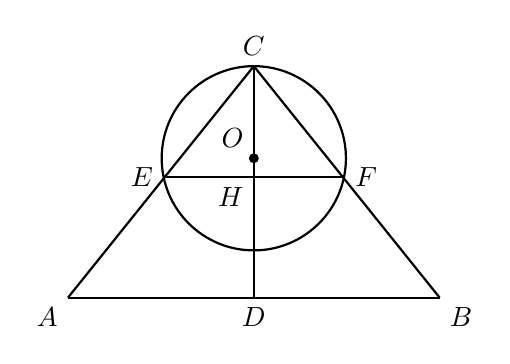
\begin{tikzpicture}[line width=0.8pt, scale=1]
  \coordinate (A) at (-2.36,0);
  \coordinate (B) at (2.36,0);
  \coordinate (C) at (0,2.94);
  \coordinate (D) at (0,0);
  \coordinate (E) at (-1.15,1.53);
  \coordinate (F) at (1.16,1.53);
  \coordinate (H) at (0,1.53);
  \coordinate (O) at (0,1.77);

  \draw (A) -- (B);
  \draw (A) -- (C);
  \draw (B) -- (C);
  \draw (E) -- (F);
  \draw (C) -- (D);
  \draw (O) circle (1.17);

  \fill (O) circle (1.8pt);

  \node[below left] at (A) {$A$};
  \node[below right] at (B) {$B$};
  \node[above] at (C) {$C$};
  \node[below] at (D) {$D$};
  \node[left] at (E) {$E$};
  \node[right] at (F) {$F$};
  \node[below left] at (H) {$H$};
  \node[above left] at (O) {$O$};
\end{tikzpicture}
\end{document}
